\documentclass[preprint]{elsarticle}
\usepackage[T1]{fontenc}
\usepackage[english]{babel}

\usepackage{amsmath, amssymb}
\usepackage{graphicx}
\usepackage{tikz}
\usetikzlibrary{arrows,automata,shapes}
\usepackage{xspace, comment}

\newcommand{\N}{\ensuremath{\mathbb{N}}\xspace}
\newcommand{\A}{\ensuremath{\mathcal{A}}\xspace}
\newcommand{\aStar}{\ensuremath{\Sigma^{*}}\xspace}
\newcommand{\aN}{\ensuremath{\Sigma^{\omega}}\xspace}
\newcommand{\aInf}{\ensuremath{\Sigma^{\infty}}\xspace}
\newcommand{\powerset}[1]{\ensuremath{\mathcal{P}\left( #1 \right)}\xspace}
\renewcommand{\L}{\ensuremath{\mathcal{L}}\xspace}
\newcommand{\Lp}{\ensuremath{\mathcal{L}'}\xspace}
\newcommand{\calF}{\ensuremath{\mathcal{F}}\xspace}
\newcommand{\calL}{\ensuremath{\mathcal{L}}\xspace}
\newcommand{\Nlanguage}{\ensuremath{\omega}-language\xspace}
\newcommand{\Nrational}{\ensuremath{\omega}-rational\xspace}
\newcommand{\aut}{\ensuremath{\mathcal{A}}\xspace}
\newcommand{\set}[1]{\ensuremath{\left\{ #1  \right\}}\xspace}
\newcommand{\card}[1]{\left| #1 \right|\xspace}
\newcommand{\Lcond}[2]{\ensuremath{\mathcal{L}^{#1}_{ #2}}\xspace} 
\newcommand{\bool}[1]{\ensuremath{\mathcal{B} \left( #1 \right)}\xspace}
\newcommand{\ie}{\emph{i.e.}\@\xspace}
\newcommand{\etc}{\emph{etc.}\@\xspace}
\newcommand{\wrt}{\emph{w.r.t.}\@\xspace}
\newcommand{\z}{\ensuremath{\mathbb{Z}}\xspace}
\newcommand{\n}{\ensuremath{\mathbb{N}}\xspace}
\newcommand{\az}{\ensuremath{A^{\mathbb{Z}}}\xspace}
\newcommand{\nuca}{\ensuremath{\nu}-CA\xspace}
\newcommand{\zrat}{\ensuremath{\zeta}-rational\xspace}
\newcommand{\R}{\ensuremath{\mathcal{R}}\xspace}
\newcommand{\cG}{\mathcal{G}}
\newcommand{\cP}{\mathcal{P}}
\newcommand{\cF}{\mathcal{F}}
\newcommand{\cL}{\mathcal{L}}
\newcommand{\cA}{\ensuremath{\mathcal{A}}\xspace}
\newcommand{\FV}[1]{\ensuremath{\mathrm{FV}\left( #1 \right)}\xspace}

\newcommand{\FA}{\ensuremath{\mathrm{FA}}\xspace}
\newcommand{\CFA}{\ensuremath{\mathrm{CFA}}\xspace}
\newcommand{\DFA}{\ensuremath{\mathrm{DFA}}\xspace}
\newcommand{\CDFA}{\ensuremath{\mathrm{CDFA}}\xspace}

\newcommand{\run}{\ensuremath{\mathrm{run}}}
\newcommand{\fin}{\ensuremath{\mathrm{fin}}}
\newcommand{\ninf}{\ensuremath{\mathrm{ninf}}}


\newcommand{\F}{\ensuremath{\mathsf{F}}\xspace}
\newcommand{\FR}{\ensuremath{\mathsf{F^{R}}}\xspace}
\newcommand{\G}{\ensuremath{\mathsf{G}}\xspace}
\newcommand{\GR}{\ensuremath{\mathsf{G^{R}}}\xspace}
\newcommand{\Fs}{\ensuremath{\mathsf{F_{\sigma}}}\xspace}
\newcommand{\FsR}{\ensuremath{\mathsf{F_{\sigma}^{R}}}\xspace}
\newcommand{\Gd}{\ensuremath{\mathsf{G}_{\delta}}\xspace}
\newcommand{\GdR}{\ensuremath{\mathsf{G_{\delta}^{R}}}\xspace}
\newcommand{\RAT}{\ensuremath{\mathsf{RAT}}\xspace}


\newdefinition{definition}{Definition}[section]
\newdefinition{remark}{\normalfont \it Remark}
\newdefinition{example}{\normalfont \it Example}
\newtheorem{theorem}{Theorem}[section]
\newtheorem{proposition}[theorem]{Proposition}
\newtheorem{lemma}[theorem]{Lemma}
\newtheorem{corollary}[theorem]{Corollary}
\newtheorem{conjecture}[theorem]{Conjecture}
\newproof{proof}{\textit{Proof}}

\makeatletter
\def\ps@pprintTitle{\let\@oddhead\@empty
  \let\@evenhead\@empty
  \def\@oddfoot{\reset@font\hfil\thepage\hfil}
  \let\@evenfoot\@oddfoot
}
\makeatother

\begin{document}

\begin{frontmatter}

\title{Acceptance conditions for \ensuremath{\omega}-languages\\ and the Borel hierarchy\tnoteref{PREV} \tnoteref{ANR}}

\tnotetext[PREV]{A preliminary version of this paper was accepted for presentation at DLT'2012 conference~\cite{dennunzio2012}.}

\tnotetext[ANR]{This work has been partially supported by the French National Research Agency project EMC (ANR-09-BLAN-0164) and by PRIN/MIUR project ``Mathematical aspects and forthcoming applications of automata and formal languages''.}

\author[Paris]{Julien Cervelle}
\ead{julien.cervelle@polytechnique.edu}

\author[Milano]{Alberto Dennunzio\corref{cor}}
\ead{dennunzio@disco.unimib.it}

\author[Nice]{Enrico Formenti\corref{cor}}
\ead{enrico.formenti@unice.fr}

\author[Giessen]{Julien Provillard}
\ead{julien.provillard@i3s.unice.fr}

\cortext[cor]{Corresponding author.}

\address[Paris]{LACL UFR de Sciences et Technologie
Universit\'e Paris-Est Cr\'eteil Val-de-Marne,
61 avenue du G\'en\'eral de Gaulle,
94010 Cr\'eteil cedex,
France}

\address[Milano]{Universit\`a degli studi di Milano-Bicocca,
Dipartimento di Informatica Sistemistica e Comunicazione,  viale
Sarca 336, 20126 Milano (Italy)}
\address[Nice]{Universit\'e Nice-Sophia Antipolis,
Laboratoire I3S, 2000 Route des Colles, 06903 Sophia Antipolis
(France)}

\address[Giessen]{
Justus-Liebig Universit\"at Gie\ss en,
Institut f\"ur Informatik,
Arndtstra\ss e 2,
35392 Gie\ss en
}



\begin{abstract}
This paper investigates acceptance conditions for finite automata recognizing -regular languages.
As a first result, we show that, under any acceptance condition that can be defined in the MSO logic, a finite automaton can recognize at
most -regular languages. Starting from this, the paper aims at
classifying acceptance conditions according to their expressive power and at finding the exact position of the classes of -languages they induced according to the Borel hierarchy.
A new interesting acceptance condition is introduced and fully characterized. A step forward is also made in
the understanding of the expressive power of  .
\end{abstract}

\begin{keyword}
finite automata \sep acceptance conditions \sep -regular languages \sep Borel hierarchy
\end{keyword}

\end{frontmatter}

\section{Introduction}

Infinite words arose as a natural extension of finite words. Their first usage (at least to our knowledge) was in symbolic dynamics.
Nowadays, they are perused in several scientific domains for example in formal specification and verification of non-terminating processes (e.g. web-servers, OS daemons, \etc) \cite{kurshan1994,kupferman2004,vardi2007}, game theory~\cite{apt2011,thomas2011}, and so on.
\smallskip

In formal software verification, for instance,  the overall state of the system
is represented by an element of some finite alphabet. Hence runs of the systems can be conveniently represented as
-words. Finite automata are often used to model the transitions of the system and their accepted
language represents the set of admissible runs of the system under observation. Acceptance conditions
on finite automata are therefore selectors of admissible runs. Main results and overall exposition about  
-languages can be found in \cite{thomas1990,staiger1997,perrin2004}.

Seminal studies about acceptance of infinite words by finite automata (\FA) have been
carried out by Richard B\"uchi while investigating monadic second order theories \cite{Buchi1960}.
A B\"uchi automaton \A  accepts an infinite word  if and only if there exists a run of \A which
passes infinitely often through a set of accepting states while reading . Later on, David Muller 
characterized runs that pass through all elements of a given set of accepting states and visit them infinitely 
often \cite{Muller1963}. Afterwards, more acceptance conditions appeared in a series of papers 
\cite{Hartmanis1967,landweber1969,Staiger1974,Moriya1988,Litovsky1997}. Each of these works was trying to
capture a particular semantic on the runs or to fill some conceptual gap.

Acceptance conditions are selectors for runs of the automaton under consideration. Of course, the set of selected
runs is also deeply influenced by the structural properties of the \FA : deterministic vs. non-deterministic, complete 
vs. non complete (see for instance \cite{Litovsky1997}).

The main purpose of this paper is to classify the expressive power of acceptance conditions in relation also with
the structural properties of the automaton. The first result bounds the research to the realm of -rational
languages: the language recognized by any \FA under any acceptance condition and \wrt to any structural property
are -rational.

Afterwards, the paper aims at positioning the classes of languages induced by the acceptance conditions found
in literature using the Borel hierarchy as a backbone. Figure~\ref{fig:hierarchy-before} illustrates the 
current state of art whilst Figure \ref{fig:hierarchy-after} summarizes the results provided by the 
present paper. Figure~\ref{fig:hierarchy-after} also illustrates the position of a new natural acceptance condition,
called \emph{\ninf}, 
introduced in the present paper to complete the panorama. This new acceptance condition declares a run of a \FA
successful if it goes through a set of accepting states only a finitely number of times or never. The underlying semantic
is that of a non-terminating process which has to definitively enter a safe state after a finite number (possibly zero) of 
exceptions (unsafe states). If some of the classes induced by \emph{\ninf} coincide with already known classes of the
Borel hierarchy, others (those induced by ) constitute a diamond strictly below .  

\section{Notations, background and basic definitions}
For any set ,  denotes the cardinality of . 
Given a finite alphabet ,  and  respectively denote the set of all finite words and the set of all infinite 
words on , respectively. As usual,   is the empty word. For any pair , 
 is the concatenation of  with .

A \emph{language} is any set . For languages ,  denote  the concatenation of  and . For a language , denote ,  and  the Kleene star of . 
The class of \emph{rational languages} 
is the smallest class of languages containing , all sets  (for ) and which is closed by union, concatenation and Kleene star.

An \emph{\Nlanguage} is any subset of . For a language , the infinite iteration of  is the \Nlanguage
 A \Nlanguage  is \emph{\Nrational} if there exist two families  and  of rational languages such that . Denote by \RAT the set of all \Nrational languages.

A \emph{finite automaton} () is a tuple  where  is a finite alphabet,  a finite set of states,  is the set of \emph{transitions},  is the \emph{initial state} and  is the \emph{acceptance table}. A  is a \emph{deterministic} finite state automaton () if  for all , . It is a \emph{complete} finite state automaton () if  for all , . We write  for a  which is both deterministic and complete. 
An (infinite) \emph{path} in a FA  is a sequence  such that  for all . The (infinite) word  is the \emph{label} of the path . A path is said to be \emph{initial} if .
\begin{definition}
Let  be a  and  an infinite path in . Define the sets
\begin{itemize}
\item
,
\item
,
\item
,
\item

\end{itemize}
as the sets of states \emph{appearing at least one time, infinitely many times,  finitely many times but at least once, and either finitely many times or never} in , respectively. 
\end{definition}

An \emph{acceptance condition} is a subset of all the initial infinite paths. The paths inside such a subset are called \emph{accepting paths}. Let  be a  and  be an acceptance condition for , a word  is \emph{accepted} by  (under condition ) if and only if it is the label of some accepting path.

Let  be the binary relation over sets such that for all sets  and ,  if and only if . 

In the sequel, we will consider acceptance conditions induced by pairs . A pair  defines an acceptance condition  on an automaton  as follows: an initial path  is  accepting if and only if there exists a set  such that  . We denote by  the \emph{language accepted by  under the acceptance condition }, \ie, the set of all words accepted by  under .

\begin{definition}
\label{classes_of_language}
For any pair  and for any finite alphabet , define the following sets 
\begin{itemize}
\item
\FA\Sigma,
\item
\DFA\Sigma,
\item
\CFA\Sigma,
\item
\CDFA\Sigma
\end{itemize}
as the classes of languages accepted by , , , and , respectively, under the acceptance condition derived by .
\end{definition}
\begin{comment}
Let  and  be two sets,  denotes the projection of words in  on the first set, \ie .


\begin{lemma}[Staiger \protect{\cite[Projection lemma]{staiger1997}}]\mbox{}\\
\label{projection}
Let .
\begin{enumerate}
\item
Let ,  be two finite alphabets.  implies 
\item
Let  be a finite alphabet.  implies there exist a finite alphabet  and a language  such that .
\end{enumerate}
\end{lemma}
\end{comment}


Some of the acceptance conditions derived by pairs  have been studied in the literature as summarized in the Table~\ref{known_results}.
\begin{table}[htb]
\begin{center}\small
\begin{tabular}{|c|c|c|c|}
\hline
&  &  &  \\
\hline
 & Landweber \cite{landweber1969} & Hartmanis\;\&\;Stearns \cite{Hartmanis1967} & Staiger\;\&\;Wagner \cite{Staiger1974}\\
\hline
 & B\"uchi \cite{Buchi1960} & Landweber \cite{landweber1969} & Muller \cite{Muller1963}\\
\hline
 & Litovski\;\&\;Staiger \cite{Litovsky1997} &  \textsc{this paper} (partially) & \textsc{this paper}\footnotemark[2]\\
\hline
 & \textsc{this paper}\footnotemark[1] & \textsc{this paper}\footnotemark[1] & \textsc{this paper}\\
\hline
\end{tabular}
\end{center}
\caption{Known results on acceptance conditions.}
\label{known_results}
\end{table}
\footnotetext[1]{These conditions have been already investigated in \cite{Moriya1988} but only in the case of complete automata with a unique set of accepting states.}
\footnotetext[2]{Only  and  are considered here. For  and  the question is still open.}

For  endowed with discrete topology and
 with the induced product topology, let , ,  and  be the collections of all closed sets, open sets, countable unions of closed set and countable intersections of open sets, respectively. For any pair  of collections of sets, denote by , , and  the  boolean closure of , the set  and the set , respectively.
These, indeed, are the lower classes of the Borel hierarchy. For more on this subject we refer the reader
to \cite{Wagner1979} or \cite{perrin2004}, for instance.

\begin{remark}
Rational and  sets are stable by projection.
\end{remark}

From now on, we fix a finite alphabet  and we omit to mention it in classes of languages.
Figure~\ref{fig:hierarchy-before} illustrates the known hierarchy of languages classes (arrows represents strict inclusions).

\begin{figure}[htb]
\begin{center}
\scalebox{0.9}{
\begin{tikzpicture}[semithick, shorten >=1pt, >=stealth']
\newcommand{\esph}{4.5}
\newcommand{\espv}{1.5}
\newcommand{\myxshift}{-20}

\tikzstyle{vertex}=[draw, shape=rectangle, font=\tiny]

\node[vertex,xshift=\myxshift] (A) at (0*\esph,0.5*\espv)
{
    
};
\node[vertex,xshift=\myxshift-28] (B) at (.7*\esph,-1*\espv)
{
    
};
\node[vertex] (C) at (-1*\esph,-\espv) 
{
    
};
\node[vertex,xshift=\myxshift] (D) at (0*\esph,-2*\espv)
{
    
};
\node[vertex] (E) at (-1*\esph,-5*\espv)
{
    
};
\node[vertex,xshift=\myxshift-36] (F) at (1*\esph,-5*\espv)
{
    
};
\node[vertex,xshift=\myxshift] (G) at (0*\esph,-6*\espv)
{
    
};
\node[vertex,xshift=\myxshift] (H) at (0*\esph,-4*\espv)
{
    
};
\node[vertex,xshift=\myxshift-36] (I) at (1*\esph,-4*\espv)
{
    
};
\node[vertex,xshift=\myxshift-8] (J) at (0.5*\esph,-3*\espv)
{
    
};
\node[vertex,xshift=\myxshift-68] (K) at (1.5*\esph,-3*\espv)
{
    
};


\draw[->] (B) -- (A);
\draw[->] (C) -- (A);
\draw[->] (D) -- (B);
\draw[->] (D) -- (C);
\draw[->] (E) -- (H);
\draw[->] (F) -- (H);
\draw[->] (H) -- (D);
\draw[->] (G) -- (E);
\draw[->] (G) -- (F);
\draw[->] (F) -- (I);
\draw[->] (H) -- (J);
\draw[->] (I) -- (J);
\draw[->] (I) -- (K);
\draw[->] (J) -- (B);
\draw[->] (K) -- (B);

\end{tikzpicture}
}
\end{center}
\caption{Currently known relations between classes of -languages recognized by \FA
according to the considered acceptance conditions and structural properties like determinism or completeness. Classes of the Borel hierarchy are typeset in bold. Arrows mean strict inclusion. Classes in the same box coincide.}
\label{fig:hierarchy-before}
\end{figure}




\section{A turn into logic}
In~\cite{Buchi1960}, B\"uchi showed that a \Nlanguage is rational if and only if it is definable in the MSO logic. We show that all the  languages recognized by one of the previously introduced acceptance condition are MSO-definable and hence rational. More generally, if an acceptance condition can be defined in the MSO logic, the languages it allows to recognize are rational.

The \emph{monadic second-order logic} (MSO logic) on the alphabet  is the logical system defined by
\begin{itemize}
\item
first-order variables , ,  \dots
\item
second-order variables (of arity 1) , ,  \dots
\item
unary relations  for ,
\item
and the binary relations ,  et .
\end{itemize}

The \emph{atomic formulas} are formulas of the form

where  and  are first-order variables,  is a second-order variable and .

The set of \emph{second-order formulas} is the smallest set which contains atomic formulas and such that for all second-order formulas  and , for all first-order variables , for all second-order variables ,

are second-order formulas.

A variable is \emph{free} in a formula if it is not introduced by a quantifier. If  is a formula, we denote by  the set of free variables which occur in . This set is recursively defined by
\begin{itemize}
\item
,
\item
,
\item
,
\item
,
\item
,
\item
 and
\item

\end{itemize}
for all first-order variables  and , for all second-order variable  and for all formulas  and .

A \emph{closed formula} is a formula without free variables. We usually denote by  a formula  where at most the variables  and  occur free.

\begin{definition}
Let  be an infinite word on , ,  and   a formula. The word  \emph{satisfies} the formula , which is denoted by

if  is true when
\begin{itemize}
\item
first-orders variables are interpreted as naturals,
\item
second-orders variables are interpreted as subsets of ,
\item
,  is interpreted as the set ,
\item
the unary relations are interpreted as the membership relations to the corresponding sets,
\item
the relations ,  et  are interpreted to be the equality, successor and order relations on , respectively,
\item
 is the interpretation of  for ,
\item
 is the interpretation of  for .
\end{itemize}
\end{definition}

\begin{definition}
Let  be a statement, the \emph{language} of  is the set

of all -words satisfying .

A \Nlanguage  is \emph{MSO-definable} if there exists a closed formula  such that .
\end{definition}

\begin{theorem}[B\"uchi \cite{Buchi1960}]
\label{th:buchi}
A \Nlanguage is \Nrational if and only if it MSO-definable.
\end{theorem}

\begin{proposition}
\label{prop:all_rat}
Let  be a \FA and  an acceptance condition derived by a pair , then  is \Nrational.
\end{proposition}

\begin{proof}
We prove that the language  is MSO-definable and we conclude by using Theorem~\ref{th:buchi}. We construct a formula  which encodes the automaton on one hand and the acceptance condition on the other hand. Let  and let  denote the elements in .  The formula describing the language is\footnote{By convention  and .}


The first three lines encode a path in .
For such a path ,  the variable~ will represent the set .
The formula

enforces the sets  to be pairwise disjoint, whereas the formula

indicates that a transition  has to be used to go from a state  to a state  by reading a letter . The formula  enforces the path to be initial because 0 is the only integer which does not have a predecessor and it has to start in the state  in this case. Finally, the formula  encodes the fact that the path is accepting according to the considered acceptance condition and its expression depends on the pair  as we will see in the following. Let  be the formula defined by

For all , the formula  would be true if and only if the previously encoded path  verifies .

We can now write the formula  depending on  by
\begin{itemize}
\item
for the relation ,

\item
for the relation ,

\item
for the relation ,
 
\end{itemize}
\qed
\end{proof}

Using the same proof, we can show that any acceptance condition which is MSO-definable only induces rational languages. We have just to change the formula  to fit to the acceptance condition.




\section{The acceptance conditions  and \textbf{} and the Borel hierarchy}

In \cite{Moriya1988},  Moriya and Yamasaki introduced two more acceptance conditions, namely  and
, and they compared them to the Borel hierarchy for the case of \CFA and \CDFA having a
unique set of accepting states. In this section, those results are generalized to \FA and \DFA and to any
set of sets of accepting states.

\begin{definition}
Given a  , the
acceptance condition  (resp. ) on   is defined as follows: an initial path  is accepting under  (resp. ) if and only if there exists a set 
 such that  (resp. ).
\end{definition}

We denote by  (resp. ) the language accepted by an automaton  under the acceptance condition  (resp. '). Similar notation as Definition~\ref{classes_of_language} are used for classes of languages.

\begin{lemma}\label{aap}\mbox{\phantom{Q}}\
T' = \set{((p,S),a,(q, S \cup \set{q})) : (p, a , q) \in T, S \in \powerset{Q}}

\calF' = \set{\set{(q, S)} : q \in Q, S \in \powerset{Q}, \exists F \in \calF, F \subseteq S} \enspace.
p' = ((p_i, \bigcup_{0 < j \leq i } \{p_j\}), x_i, (p_{i+1},\bigcup_{0 < j \leq i+1} \{p_j\}))_{i \in \N}
-4ex]
\begin{enumerate}
\item
\enspace, 
\item
\enspace, 
\item
\enspace,
\item
\enspace.
\end{enumerate}
\end{lemma}

\begin{proof}
We are going to show that for any   there exists an   such that  and  is deterministic (resp. complete) if  is deterministic (resp. complete). 

Let  where . Clearly,  is deterministic (resp. complete) if  is deterministic (resp. complete). Moreover,  if and only if there exist an initial path  in  with label  and a set  such that , or, equivalently,  there exist an initial path  in  with label  and a set  such that , \ie, if and only if .\qed
\end{proof}

\begin{lemma}\label{aprime}\mbox{\phantom{Q}}\
T' & =  \left\{((p,S),a,(q, S \cup \set{q})) : (p, a , q) \in T, S \in \powerset{Q}, \exists F \in \calF, F \not\subseteq S \cup \set{q}\right\} \\
 & \bigcup  \set{((p,S),a,\bot) : S \in \powerset{Q}, \exists q \in Q, (p, a , q) \in T, \forall F \in \calF, F \subseteq S \cup \set{q}} \\
 & \bigcup  \set{(\bot, a, \bot) : a \in \Sigma} \enspace.
-4ex]
\begin{enumerate}
\item
\enspace,
\item
\enspace,
\item
\enspace,
\item
\enspace.
\end{enumerate}
\end{lemma}

\begin{proof}
We are going to show that for any   there exists an automaton   such that  and  is deterministic (resp. complete) if  is deterministic (resp. complete). 

Let  where , , and 


Then,  is deterministic (resp. complete) if  is deterministic (resp. complete).
Moreover, 
 if and only if there exists an initial path  in  with label  and a set  such that  iff there exists an initial path  in  with label  such that  for all , \ie, if and only if .\qed
\end{proof}

The following result places the classes of langages characterized by  and 
\wrt the Borel hierarchy.

\begin{theorem}\mbox{\phantom{Q}}\ 
\Lcond{\mathbb{L}}{\A} = \Lcond{(\ninf, \subseteq)}{\A'} \text{ and } \Lcond{(\ninf, \subseteq)}{\A} = \Lcond{\mathbb{L}}{\A'} \\ (\text{resp. } \Lcond{\mathbb{L'}}{\A} = \Lcond{(\ninf, \sqcap)}{\A'} \text{ and } \Lcond{(\ninf, \sqcap)}{\A} = \Lcond{\mathbb{L'}}{\A'})\enspace.
\Lcond{\mathbb{L}}{\A} = \bigcup_{F \in \calF} \bigcap_{q \in F} \Lcond{(\inf, \sqcap)}{\A_{q}}\enspace.
T' & = \set{((p,S),a,(q, (S \cup \set{q}) \cap F)) : (p, a , q) \in T, (p,S) \neq (f,F)} \\
 & \bigcup  \set{((f,F),a,(q,\emptyset)) : (f, a , q) \in T}\enspace.
(p_0, a, p_1), (p_1, b, p_2),  \ldots (p_i, b, p_{i+1}),\ldots  (p_{j-1}, b, p_j=p_{i})\ldots(p'_0, b, p'_1), \ldots (p'_{l-1}, b, p'_l=f=p_h),  \ldots (p_n, b, p_{n+1}),(p_{n+1}, a, p_{n+2})\ldots(p_0, a, p_1), \ldots (p_{n-1}, a, p_n),  (p_n, b, p_{n+1}),  (p_{n+1}, a, p_{n+2})\ldots(p'_0, b, p'_1), \ldots (p'_{n-1}, b, p'_n),  (p'_n, b, p'_{n+1}), (p_{n+1}, a, p_{n+2})\ldots(p'_0, b, p'_1), \ldots (p'_{k-1}, b, p'_k=f=p_h),  (p_{h}, a, p_{h+1}),\ldots (p_{j-1}, a, p_{j}=p_i)\ldots
\CDFA(\ninf,=) = \DFA(\ninf,=) = \CFA(\ninf,=) = \FA(\ninf,=) = \RAT\enspace.

\DFA(\fin,\subseteq) = \CDFA(\fin,\subseteq) \text{ and }\FA(\fin,\subseteq) = \CFA(\fin,\subseteq)\enspace,\\
\DFA(\fin,=) = \CDFA(\fin,=) \text{ and }\FA(\fin,=) = \CFA(\fin,=)\enspace.

T'  =  T & \cup \set{(p,a,\bot) : p \in Q, a \in \Sigma, \forall q \in Q, (p,a,q) \not\in T} \cup \set{(\bot, a, \bot') : a \in \Sigma}\\
&\cup \set{(\bot', a, \bot') : a \in \Sigma}
T' = T \cup \set{(p,a,(q,p)) : (p,a,q) \in T} \cup \set{((p_1, p_2), a, q) : (p_1,a,q) \in T, p_2 \in Q}\calF' = \set{F \smallsetminus \set{p_2} \cup \set{(p_1,p_2)} : p_1 \in Q, F \in \powerset{Q}, \exists X \in \calF, p_2 \in X}\enspace.\A = (\set{a,b}, \set{q_0, q_1,q_2,q_3,q_4,q_5}, T, q_0, \set{\emptyset, \set{q_2}, \set{q_3,q_4}})\enspace,
\bigcup_{S, S \subseteq Q, \exists F \in \calF, S \smallsetminus S' \subseteq F}
\left(\Lcond{(\run,\subseteq)}{\A_S} \cap \bigcap_{q \in S'} \Lcond{(\inf,\sqcap)}{\A_{\set{q}}}\right) \enspace,

x \in \Lcond{(\run,\subseteq)}{\A_S} \cap \bigcap_{q \in S'} \Lcond{(\inf,\sqcap)}{\A_{\set{q}}} \subseteq \calL \enspace.

Conversely, we prove that . Let , by determinism, there exists a path  in  labeled by  such that there exist ,  with  such that  is accepting for  under  and for  under  for all . The path  verifies ,  and then . Finally,  is accepting for  under  and .

 For all ,  and . As  is stable by finite intersection and union, .

\qed
\end{proof}
\begin{comment}
\begin{corollary}
.
\end{corollary}

\begin{proof}
Combine Lemma~\ref{projection} and Proposition~\ref{lem_fin_subset_det_Fsigma}.\qed
\end{proof}
\end{comment}
\begin{figure}[htb]
\begin{center}
\scalebox{0.9}{
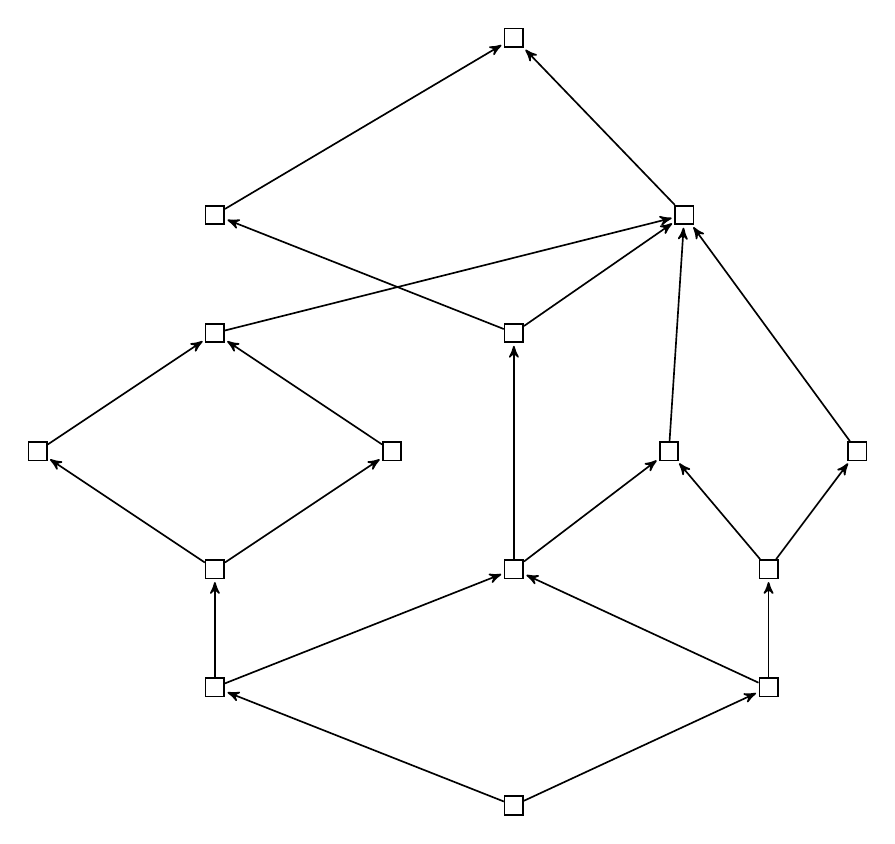
\begin{tikzpicture}[semithick, shorten >=1pt, >=stealth']
\newcommand{\esph}{4.5}
\newcommand{\espv}{1.5}
\newcommand{\myxshift}{-20}

\tikzstyle{vertex}=[draw, shape=rectangle, font=\tiny]

\node[vertex,xshift=\myxshift] (A) at (0*\esph,0.5*\espv)
{
    
};
\node[vertex,xshift=\myxshift-28] (B) at (.7*\esph,-1*\espv)
{
    
};
\node[vertex] (C) at (-1*\esph,-\espv) 
{
    
};
\node[vertex,xshift=\myxshift] (D) at (0*\esph,-2*\espv)
{
    
};
\node[vertex] (E) at (-1*\esph,-5*\espv)
{
    
};
\node[vertex,xshift=\myxshift-36] (F) at (1*\esph,-5*\espv)
{
     
};
\node[vertex,xshift=\myxshift] (G) at (0*\esph,-6*\espv)
{
    
};
\node[vertex,xshift=\myxshift] (H) at (0*\esph,-4*\espv)
{
    
};
\node[vertex,xshift=\myxshift-36] (I) at (1*\esph,-4*\espv)
{
    
};
\node[vertex,xshift=\myxshift-8] (J) at (0.5*\esph,-3*\espv)
{
    
};
\node[vertex,xshift=\myxshift-68] (K) at (1.5*\esph,-3*\espv)
{
    
};
\node[vertex] (L) at (-1*\esph,-4*\espv)
{
    
};
\node[vertex] (M) at (-0.5*\esph,-3*\espv)
{
    
};
\node[vertex] (N) at (-1.5*\esph,-3*\espv)
{
    
};
\node[vertex] (O) at (-1*\esph,-2*\espv)
{
    
};


\draw[->] (B) -- (A);
\draw[->] (C) -- (A);
\draw[->] (D) -- (B);
\draw[->] (D) -- (C);
\draw[->] (E) -- (H);
\draw[->] (F) -- (H);
\draw[->] (H) -- (D);
\draw[->] (G) -- (E);
\draw[->] (G) -- (F);
\draw[->] (F) -- (I);
\draw[->] (H) -- (J);
\draw[->] (I) -- (J);
\draw[->] (I) -- (K);
\draw[->] (J) -- (B);
\draw[->] (K) -- (B);
\draw[->] (E) -- (L);
\draw[->] (L) -- (M);
\draw[->] (L) -- (N);
\draw[->] (M) -- (O);
\draw[->] (N) -- (O);
\draw[->] (O) -- (B);

\end{tikzpicture}
}
\end{center}
\caption{The completion of Figure~\ref{fig:hierarchy-before} with the results in the paper.
Classes of the Borel hierarchy are typeset in bold. Arrows mean strict inclusion. Classes in the same box coincide.}
\label{fig:hierarchy-after}
\end{figure}



\section{Conclusions}

In this paper we have studied the expressivity power of acceptance conditions for finite automata.
Three new classes have been fully characterized. For a fourth one, partial results are given.
In particular,  provides four distinct new classes of languages (see the diamond
in the left part of Figure \ref{fig:hierarchy-after}), all other acceptance conditions considered tend
to give (classes of) languages populating known classes.

In literature, other well-known acceptance conditions exists for example Rabin, Strett or Parity 
conditions. These last ones have not been taken into account in the present paper since it is known
that they are equivalent to Muller's condition. 

Several research directions should be further explored but at least two seems the more promising ones.
First, to complete the characterization of . Moreover, the exact position of  
in the hierarchy given so far is still under investigation.

Second, to study the closure properties of the the new classes of languages introduced in the paper  and 
verify if they cram the known classes or if they add new elements to Figure \ref{fig:hierarchy-after}.

\bibliographystyle{plain}
\bibliography{references}

\end{document}
